\documentclass[floatsintext,man]{apa6}

\usepackage{amssymb,amsmath}
\usepackage{ifxetex,ifluatex}
\usepackage{fixltx2e} % provides \textsubscript
\ifnum 0\ifxetex 1\fi\ifluatex 1\fi=0 % if pdftex
  \usepackage[T1]{fontenc}
  \usepackage[utf8]{inputenc}
\else % if luatex or xelatex
  \ifxetex
    \usepackage{mathspec}
    \usepackage{xltxtra,xunicode}
  \else
    \usepackage{fontspec}
  \fi
  \defaultfontfeatures{Mapping=tex-text,Scale=MatchLowercase}
  \newcommand{\euro}{€}
\fi
% use upquote if available, for straight quotes in verbatim environments
\IfFileExists{upquote.sty}{\usepackage{upquote}}{}
% use microtype if available
\IfFileExists{microtype.sty}{\usepackage{microtype}}{}

% Table formatting
\usepackage{longtable, booktabs}
\usepackage{lscape}
% \usepackage[counterclockwise]{rotating}   % Landscape page setup for large tables
\usepackage{multirow}		% Table styling
\usepackage{tabularx}		% Control Column width
\usepackage[flushleft]{threeparttable}	% Allows for three part tables with a specified notes section
\usepackage{threeparttablex}            % Lets threeparttable work with longtable

% Create new environments so endfloat can handle them
% \newenvironment{ltable}
%   {\begin{landscape}\begin{center}\begin{threeparttable}}
%   {\end{threeparttable}\end{center}\end{landscape}}

\newenvironment{lltable}
  {\begin{landscape}\begin{center}\begin{ThreePartTable}}
  {\end{ThreePartTable}\end{center}\end{landscape}}




% The following enables adjusting longtable caption width to table width
% Solution found at http://golatex.de/longtable-mit-caption-so-breit-wie-die-tabelle-t15767.html
\makeatletter
\newcommand\LastLTentrywidth{1em}
\newlength\longtablewidth
\setlength{\longtablewidth}{1in}
\newcommand\getlongtablewidth{%
 \begingroup
  \ifcsname LT@\roman{LT@tables}\endcsname
  \global\longtablewidth=0pt
  \renewcommand\LT@entry[2]{\global\advance\longtablewidth by ##2\relax\gdef\LastLTentrywidth{##2}}%
  \@nameuse{LT@\roman{LT@tables}}%
  \fi
\endgroup}


  \usepackage{graphicx}
  \makeatletter
  \def\maxwidth{\ifdim\Gin@nat@width>\linewidth\linewidth\else\Gin@nat@width\fi}
  \def\maxheight{\ifdim\Gin@nat@height>\textheight\textheight\else\Gin@nat@height\fi}
  \makeatother
  % Scale images if necessary, so that they will not overflow the page
  % margins by default, and it is still possible to overwrite the defaults
  % using explicit options in \includegraphics[width, height, ...]{}
  \setkeys{Gin}{width=\maxwidth,height=\maxheight,keepaspectratio}
\ifxetex
  \usepackage[setpagesize=false, % page size defined by xetex
              unicode=false, % unicode breaks when used with xetex
              xetex]{hyperref}
\else
  \usepackage[unicode=true]{hyperref}
\fi
\hypersetup{breaklinks=true,
            pdfauthor={},
            pdftitle={Child language experience in a Tseltal Mayan village},
            colorlinks=true,
            citecolor=blue,
            urlcolor=blue,
            linkcolor=black,
            pdfborder={0 0 0}}
\urlstyle{same}  % don't use monospace font for urls

\setlength{\parindent}{0pt}
%\setlength{\parskip}{0pt plus 0pt minus 0pt}

\setlength{\emergencystretch}{3em}  % prevent overfull lines


% Manuscript styling
\captionsetup{font=singlespacing,justification=justified}
\usepackage{csquotes}
\usepackage{upgreek}

 % Line numbering
  \usepackage{lineno}
  \linenumbers


\usepackage{tikz} % Variable definition to generate author note

% fix for \tightlist problem in pandoc 1.14
\providecommand{\tightlist}{%
  \setlength{\itemsep}{0pt}\setlength{\parskip}{0pt}}

% Essential manuscript parts
  \title{Child language experience in a Tseltal Mayan village}

  \shorttitle{Child language experience in a Tseltal Mayan village}


  \author{Marisa Casillas\textsuperscript{1}, Penelope Brown\textsuperscript{1}, \& Stephen C. Levinson\textsuperscript{1}}

  % \def\affdep{{"", "", ""}}%
  % \def\affcity{{"", "", ""}}%

  \affiliation{
    \vspace{0.5cm}
          \textsuperscript{1} Max Planck Institute for Psycholinguistics  }

  \authornote{
    Correspondence concerning this article should be addressed to Marisa
    Casillas, P.O. Box 310, 6500 AH Nijmegen, The Netherlands. E-mail:
    \href{mailto:Marisa.Casillas@mpi.nl}{\nolinkurl{Marisa.Casillas@mpi.nl}}
  }


  \abstract{Enter abstract here. Each new line herein must be indented, like this
line.}
  \keywords{Child-directed speech, Linguistic input, Non-WEIRD, Vocal maturity, Turn
taking \\

    \indent Word count: X
  }





\usepackage{amsthm}
\newtheorem{theorem}{Theorem}[section]
\newtheorem{lemma}{Lemma}[section]
\theoremstyle{definition}
\newtheorem{definition}{Definition}[section]
\newtheorem{corollary}{Corollary}[section]
\newtheorem{proposition}{Proposition}[section]
\theoremstyle{definition}
\newtheorem{example}{Example}[section]
\theoremstyle{definition}
\newtheorem{exercise}{Exercise}[section]
\theoremstyle{remark}
\newtheorem*{remark}{Remark}
\newtheorem*{solution}{Solution}
\begin{document}

\maketitle

\setcounter{secnumdepth}{0}



\section{Introduction}\label{intro}

A great deal of work in developmental language science revolves around
one central question: What linguistic evidence (i.e., what types and how
much) is needed to support first language acquisition? In pursuing this
topic, many researchers have fixed their sights on child-directed speech
(CDS), showing that it is linguistically distinctive
(REFS)\textbf{{[}TASK 00: Add missing references{]}}, interactionally
rich (REFS), preferred by infants (REFS), and---perhaps most
importantly---facilitates word learning (REFS). By all appearances, CDS
is an essential component for acquiring a first language. Yet
ethnographic reports from a number of traditional, non-Western
communities suggest that children easily acquire their community's
language(s) with little or no CDS (REFS). If so, CDS may not be
essential for learning language; just useful for facilitating certain
aspects of language development. In this paper we investigate the
language environment and early development of 10 Tseltal Mayan children
growing up in a community where past research has suggested that
caregivers use little CDS with infants and young children (REFS Brown).

\subsection{Child-directed speech}\label{intro-cds}

The amount of CDS children hear influences their language development,
particularly their vocabulary (REFS). For example, \textbf{{[}TASK 01:
Add examples of input-vocab link{]}}. CDS has also been linked to young
children's speed of lexical retrieval (REFS Weisleder; LuCiD) and
syntactic development (REFS Huttenlocher). \textbf{{[}TASK 02: Read
Huttenlocher and add details here{]}}. The conclusion drawn from much of
this work is that CDS is an ideal register for learning
words---especially concrete nouns and verbs---because it is tailored to
maximize a child's moment-to-moment interest and understanding (REFS).
Indeed, even outside of first-person interaction, infants and young
children prefer listening to CDS over adult-directed speech (REFS
ManyBabies, etc.), suggesting that CDS is useful in catching,
maintaining, and focusing children's attention. There are, however, a
few significant caveats to the body of work relating CDS quantity to
language development.

First, while there is overwhelming evidence linking CDS quantity to
vocabulary size, links to grammatical development are more scant (REFS:
Huttenlocher; Frank et al.). While the advantage of CDS for referential
word learning is clear, it is less obvious how CDS facilitates syntactic
learning. \textbf{{[}TASK 03: Add argument from Yurovsky paper +
refrences therein{]}} On the other hand, there is a wealth of evidence
that both children and adults' syntactic knowledge is highly lexically
specified (REFS), and that, crosslinguistically, children's vocabulary
size is one of the most robust predictors of their early syntactic
development (REFS). In short, what is good for the lexicon may also be
good for syntax. For now, however, the link between CDS and other
aspects of grammatical development still needs to be more thoroughly
tested.

A second caveat is that most work on CDS quantity uses summary measures
that average over the ebb and flow of interaction (e.g., proportion
CDS). In both child and adult interactions, verbal behaviors are highly
structured: while some occur at fairly regular intervals
(\enquote{periodic}), others occur in shorter, more intense bouts
separated by long periods of inactivity (\enquote{bursty} REFS Abney
2018 bursts and lulls, see also fusaroli et al. 2014 synergy). For
example, Abney and colleagues (2016 REFS) found that, across multiple
time scales of daylong recordings, both infants' and adults' vocal
behavior was clustered. Focusing on lexical development, Blasi and
colleagues (REFS in prep) also found that nouns and verbs were used
burstily in child-proximal speech across all six of the languages in
their typologically diverse sample. Infrequent words were somewhat more
bursty overall, leading them to propose that burstiness may play a key
and universal role in acquiring otherwise-rare linguistic units (see
also REFS in prep from
ICIS).\footnote{But see Drew and Bergelson (REFS in preparation), who find that the highest-frequency nouns used in CDS and children's own speech were relatively more bursty than other nouns.}
Experiment-based work also shows that two-year-olds learn novel words
better from a massed presentation of object labels versus a distributed
presentation (Schwab and Lew-Williams (2016) REFS; but see REFS Ambridge
et al., 2006; Childers and Tomasello, 2002). Structured temporal
characteristics in children's language experience imply new roles for
attention and memory in language development. By that token, we should
begin to investigate the link between CDS and linguistic development
with more nuanced measures of how CDS is distributed.

Finally, prior work has typically focused on Western (primarily North
American) populations, limiting our ability to generalize these effects
to children acquiring language worldwide (REFS: WEIRD; Lieven, 1994).
While we do gain valuable insight by looking at \emph{within-population}
variation (e.g., REFS), we can more effectively find places where our
assumptions break down by studying \emph{new} populations. Linguistic
anthropologists working in non-Western communities have long reported
that caregiver interaction styles vary immensely from place to place,
with some caregivers using little or no CDS to young children (REFS
Gaskins, 2006). Children in these communities reportedly acquire
language with \enquote{typical}-looking benchmarks. For example, they
start pointing (REFS Liszkowski et al., 2012; but see Salomo \&
Liszkowski, 2013) and talking (REFS Rogoff et al., 2003?; Brown??)
around the same time we would expect for Western middle-class infants.
These findings have had little impact on mainstream theories of word
learning and language acquisition, partly due to a lack of directly
comparable measures (Brown, 2014). If, however, these children indeed
acquire language without delay despite little or no CDS, we must
reconsider what kind of linguistic evidence is necessary for children to
learn language.

\subsection{Language development in non-WEIRD
communities}\label{intro-nonweird}

To our knowledge, only a handful of researchers have used methods from
developmental psycholinguistics to describe the language environments
and linguistic development of children growing up in traditional,
non-Western communities. We briefly highlight two recent efforts along
these lines, but see Mastin and Vogt (REFS 2016) and Cristia et al.
(2017) for more examples.

Scaff, Cristia, and colleagues (REFS 2017; in preparation) have used a
number of methods to estimate how much speech children hear in a Tsimane
forager-horticulturalist population in the Bolivian lowlands. Their
daylong recordings show that Tsimane children between 0;6 and 6;0 hear
\textasciitilde{}5 minutes of CDS per hour, regardless of their age (but
see Cristia et al., 2017). For comparison, children from North American
homes between ages 0;3 and 3;0 are estimated to hear \textasciitilde{}11
minutes of CDS per hour in daylong recordings (REFS: Bergelson,
Casillas, et al., see also REFS the newer Tamis-LeMonda paper; maybe
give estimates w/ age ranges for each??). Tsimane children also hear
\textasciitilde{}10 minutes of other-directed speech per hour (e.g.,
talk between adults) compared to the \textasciitilde{}7 minutes per hour
heard by North American children (REFS Bergelson, Casillas, et al.).
This difference may be attributable to the fact that the Tsimane live in
extended family clusters of 3--4 households, so speakers are typically
in close proximity to 5--8 other people (REFS Cristia et al., 2017).

Laura Shneidman and colleagues (REFS; 2010; 2012) analyzed speech from
1-hour at-home video recordings of children between ages 1;0 and 3;0 in
two communities: Yucatec Mayan (Southern Mexico) and North American (a
major U.S. city). Their analyses yielded four main findings: compared to
the American children, (a) the Yucatec children heard many fewer
utterances per hour, (b) a much smaller proportion of the utterances
they heard were \emph{child-directed}, (c) the proportion of utterances
that were child-directed increased dramatically with age, matching U.S.
children's by 3;0 months, and (d) most of the added CDS came from other
children (e.g., older siblings and cousins). They also demonstrated that
the lexical diversity of the CDS they hear at 24 months---particularly
from adult speakers---predicted children's vocabulary knowledge at 35
months.

These groundbreaking studies establish a number of important findings:
First, children in each of these communities appear able to acquire
their languages with relatively little CDS. Second, CDS might become
more frequent as children get older, though this could largely be due to
speech from other children. Finally, despite these differences, CDS from
adults may still be the most robust predictor of vocabulary growth.

\subsection{The current study}\label{intro-currentstudy}

We examine the early language experience of 10 Tseltal Mayan children
under age 3;0. Prior ethnographic work suggests that Tseltal caregivers
do not frequently speak directly to their children until the children
themselves begin speaking (REFS: Brown??). Nonetheless, Tseltal children
develop language with no apparent delays. Tseltal Mayan language and
culture has much in common with the Yucatec Mayan communities Shneidman
reports on (REFS: 2010 + add other stuff that's not nec lg), allowing us
to compare differences in child language environments between the two
sites more directly than before.\textbackslash{}footnote\{For a review
of comparative work on language socialization in Mayan cultures, see Pye
(2017).) We provide more details on this community and dataset in the
\protect\hyperlink{methods}{Methods section}.

Similar to previous work, we estimated how much speech children
overheard, how much was directed to them, and how those quantities
changed with age. To this foundation we added new sampling techniques
for investigating variability in children's speech environments within
daylong recordings. We also analyzed children's early vocal productions,
examining both the overall developmental trajectory of their vocal
maturity and how their vocalizations are influenced by CDS.

Based on prior work, we predicted that Tseltal Mayan children hear
little CDS, that the amount of CDS they hear increases with age, that
most CDS comes from other children, and that, despite this, Tseltal
Mayan children reach speech production benchmarks on par with Western
children. We additionally predicted that children's language
environments would be bursty---that brief, high-intensity interactions
would be sparsely distributed throughout the day, accounting for the
majority of children's daily CDS---and that children's responsiveness
and vocal maturity would be maximized during these moments of
high-intensity interaction.

\hypertarget{methods}{\section{Methods}\label{methods}}

\subsection{Community}\label{methods-community}

The children in our dataset (REFS: Casillas HomeBank) come from a
small-scale, subsistence farming community in the highlands of Chiapas
in Southern Mexico. The vast majority of children grow up speaking
Tseltal monolingually at home. Primary school is conducted in Tseltal,
but secondary and further education is primarily conducted in Spanish.
Nuclear families are often large (5+ children) and live in patrilineal
clusters. Nearly all families grow staple crops such as corn and beans,
but also bananas, chilies, squash, coffee, and more. Household and
farming work is divided among men, women, and older children. Women do
much of the daily cleaning and food preparation, but also frequently
work in the garden, haul water and firewood, and do other physical
labor. A few community members---both men and women---earn incomes as
teachers and shopkeepers but are still expected to regularly contribute
to their family's household work.

More than forty years of ethnographic work by the second author has
reported that Tseltal children's language environments are
non-child-centered and non-object-centered (REFS). During their waking
hours, Tseltal infants are typically tied to their mother's back while
she goes about her work for the day. Infants receive very little direct
speech until they themselves begin to initiate interactions, usually as
they approach their first birthdays. Even then, interactional exchanges
are often brief or non-verbal (e.g., object exchange routines) and take
place within a multi-participant context (Brown 2011; 2014). Rarely is
attention given to words and their meanings, even when objects are
central to the activity. Instead, interactions tend to focus on
appropriate actions and responses, and young children are socialized to
attend to the interactions taking place around them (REFS see also
Rogoff and de Leon).

Young children are often cared for by other family members, especially
older siblings. Even when not on their mother's back, infants are rarely
put on the ground, so they can't usually pick up the objects around them
until they are old enough to walk. Toys are scarce and books are
vanishingly rare, so the objects children do get their hands on tend to
be natural or household objects (e.g., rocks, sticks, spoons, baskets,
etc.). By age five, most children are competent speakers who engage
daily in chores and caregiving of their younger siblings. The Tseltal
approach to caregiving is similar to that described for other Mayan
communities (e.g., REFS Rogoff, Gaskins, de Leon, Shneidman).

\subsection{Corpus}\label{methods-corpus}

The current data come from the Casillas HomeBank Corpus (REFS HomeBank),
which includes daylong recordings and other developmental language data
from more than 100 children under 4;0 across two indigenous, non-WEIRD
communities: the Tseltal Mayan community described here and a Papua New
Guinean community described elsewhere (REFS).

\emph{{[}TASK 06: Check these demographic data again{]}} The Tseltal
data, primarily collected in 2015, include recordings from 55 children
born to 43 mothers. The families in our dataset typically only had 2--3
children (median = 2; range = 1--9), due to the fact that the
participating families come from a young subsample of the community
(mothers: mean = 26.9 years; median = 25.9; range = 16.6--43.8 and
fathers: mean = 30.5; median = 27.6; range = 17.7---52.9). On average,
mothers were 20.1 years old when they had their first child (median =
19; range = 12--27), with a following inter-child interval of 3.04 years
(median = 2.8; range =
1--8.5).\footnote{These estimates do not include miscarriages and/or children who passed away.}.
As a result, 26\% of the participating families had two children under
4;0.

Extended households, defined in our dataset as the group sharing a
kitchen or other primary living space, ranged between between 3 and 15
people (mean = NN; median = NN). Although 30.9\% of the target children
are first-born, they were rarely the only child in their extended
household. Caregiver education is one (imperfect) measure of contact
with Western culture. Most mothers had finished primary school, with
many also having completed secondary school (range = no
schooling--university). Most fathers had finished secondary school, with
many having also completed preparatory school (range = no
schooling--university). Owing in large part to patrilineal (i.e., father
to son) land inheritance, 93\% of the fathers grew up in the village
where the recordings took place, while only 53\% of the mothers did.

\subsubsection{Recordings}\label{methods-corpus-recs}

Methods for estimating the quantity of speech that children hear have
advanced significantly in the past two decades, with long-format at-home
audio recordings quickly becoming the new standard (e.g., with the
LENA\textsuperscript{®} system; REFS). These recordings capture a wider
range of the linguistic patterns children hear as they participate in
different activities with different speakers over the course of their
day. In longer, more naturalistic recordings, caregivers also tend to
use less CDS (REFS Tamis-LeMonda). The result is greater confidence that
the estimated CDS characteristics are representative of what the child
typically hears at home.

We used a novel combination of a lightweight stereo audio recorder
(Olympus\textsuperscript{®} WS-832) and wearable photo camera (Narrative
Clip 1\textsuperscript{®}) fitted with a fish-eye lens, to track
children's movements and interactions over the course of a 9--11-hour
period in which the experimenter was not present. Each recording was
made during a single day at home in which the recorder and/or camera was
attached to the child. Ambulatory children wore both devices on an
elastic vest. Non-ambulatory children wore the recorder in a onesie
while their primary caregiver wore the camera on an elastic vest
\emph{Figure 1} \emph{{[}TASK 07: Make figure{]}}. The camera was set to
take photos at 30-second intervals and was synchronized to the audio in
post-processing to create video of the child's daylong
recording.\footnote{Documentation for recording set-up and scripts for post-processing are available at *[TASK 08: Link to relevant docs]*}

\subsection{Data selection and annotation}\label{methods-samples}

We annotated video clips from 10 of the 55 children's recordings. We
chose these 10 recordings to maximize variance in three demographic
variables: child age (0--3;0), child sex, and maternal education. The
sample is summarized in \emph{Table 1} \emph{{[}TASK 09: Make table{]}}.
We then selected one hour's worth of non-overlapping clips from each
recording in the following order: nine randomly selected 5-minute clips,
five 1-minute clips manually selected as the top \enquote{turn-taking}
minutes of the recording, five 1-minute clips manually selected as the
top \enquote{vocal activity} minutes of the recording, and one, manually
selected 5-minute extension of the best 1-minute sample \emph{FIGURE ??}
\emph{{[}TASK 10: Add figure of recording times with samples highlighted
for the 10 recs{]}}. We created these different subsamples of each day
to measure properties of (a) children's \emph{average} language
environments (random samples) and (b) their \emph{most input-dense}
language environments (turn-taking samples). The third sample
(high-activity) gave us insight into children's productive speech
abilities.

The turn-taking and high-activity clips were chosen by two trained
annotators (the first author and a student assistant) who listened to
each recording in its entirety at 1--2x speed while actively taking
notes about potentially useful clips. Afterwards, the first author
reviewed the list of candidate clips, listened again to each one (at 1x
speed, multiple repetitions), and chose the best five 1-minute samples
for each of the two types of activity. Good turn-taking activity was
defined as at closely timed sequences of contingent vocalization between
the target child and at least one other person (i.e., frequent
vocalization exchanges). The \enquote{best} turn-taking clips were
chosen because they had the most and most clear turn-switching activity
between the target child and the other speaker(s). Good vocal activity
clips were defined as clips in which the target child produced the most
and most diverse spontaneous (i.e., not imitative) vocalizations. The
\enquote{best} vocal activity clips were chosen for representing the
most linguistically mature and/or diverse vocalizations made by the
child over the day. All else being equal, candidate clips were
prioritized when they contained less background noise or featured
speakers and speech that were not otherwise frequently represented
(e.g., CDS from older males). The best turn-taking clips and vocal
activity clips often overlapped; turn-taking clips were selected from
the list of candidates first, and then vocal-activity clips were chosen
from the remainder.

\begin{figure}
\centering
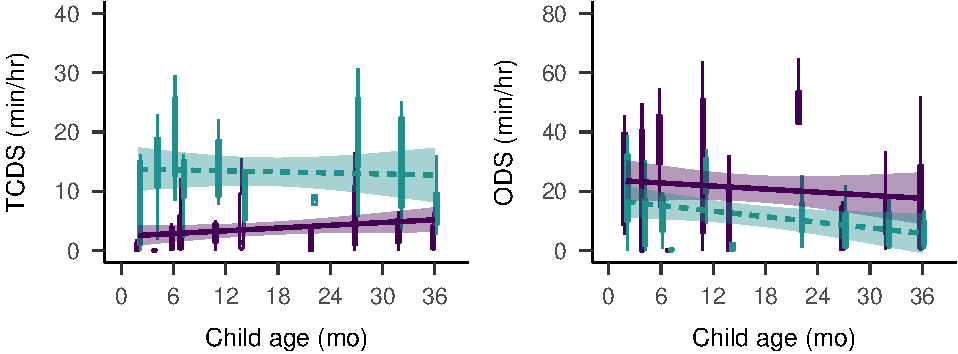
\includegraphics{Tseltal-CLE_files/figure-latex/fig1-1.pdf}
\caption{\label{fig:fig1}Recording duration (black line) and sampled clips
(colored boxes) for each recording analyzed, sorted by child age.}
\end{figure}

Each video clip was transcribed and annotated in ELAN (REFS) using the
ACLEW Annotation Scheme (REFS) by the first author and a native speaker
of Tseltal who lives in the community and knows most of the recorded
families personally. At the time of writing, NN\% \emph{{[}TASK XX: Fill
in before submitting{]}} of the clips have been reviewed by a second
native Tseltal speaker. The annotations include the transcription of
(nearly) all hearable utterances in Tseltal, a loose translation of each
utterance into Spanish, vocal maturity measures of each target child
utterance (non-linguistic vocalizations/non-canonical babbling/non-word
canonical babbling/single words/multiple words), and addressee
annotations for all non-target-child utterances
(target-child-directed/other-child-directed/adult-directed/adult-and-child-directed/animal-directed/other-speaker-type-directed).\footnote{Full documentation, including training materials, for the ACLEW Annotation Scheme can be found at *[TASK 11: Add OSF link]*.}
We exported each ELAN file as tab-separated values for analysis.

\subsubsection{Why vocal maturity?}\label{why-vocal-maturity}

\emph{{[}TASK 12: Missing paragraph!!{]}}

\subsection{Data analysis}\label{methods-analysisinfo}

In what follows, we first describe quantitative characteristics of
children's speech environments, as captured by the 9 randomly selected
five-minute clips for each child. We report five measures:
target-child-directed speech (TCDS) and other-directed speech (ODS)
minutes per hour, the number of target-child-to-other (TC--O) and
other-to-target-child (O-TC) turn transitions per minute, and the
duration of the target child's interactional sequences in seconds. We
then briefly review these same speech environment characteristics for
the 5--6 one- or five-minute turn-taking clips\footnote{The turn-taking
  clips included in this analysis are: the 5 one-minute turn-taking
  clips and also the five-minute \enquote{extension} clip for that
  recording if it was an extension of a turn-taking clip.}, as
representative \enquote{peak} interactional moments in the day and
investigate how many minutes in the day are likely to have these
characteristics.

\section{Results}\label{results}

\emph{{[}TASK 14: change fits in the figures to reflect model
estimates{]}}

\subsection{Data analysis}\label{data-analysis}

Unless otherwise stated, all analyses were conducted with generalized
linear mixed-effects regressions using the glmmTMB package and all plots
are generate with ggplot2 in R (Brooks et al., 2017a; R Core Team, 2018;
Wickham, 2009).\footnote{The data and analysis code are freely available
  on the web ({[}retracted for review{]}), as is a summary of the
  results which will be updated as more transcriptions become available
  ({[}retracted for review{]}).} Notably, all five speech environment
measures are restricted to non-negative values (min/hr, turn
transitions/min, and duration in seconds), with a subset of them also
displaying extra cases of zero in the randomly sampled clips (min/hr,
turn transitions/min; e.g., when the child is napping). The consequence
of these boundary restrictions is that the variance of the distributions
becomes non-gaussian (i.e., a long right tail). We account for this
issue by using negative binomial regression, whish is useful for
overdispersed count data (Brooks et al., 2017b; Smithson \& Merkle,
2013). When extra cases of zero are present due to, e.g., no speakers
being present, we used a zero-inflation negative binomial regression,
which creates two models: (a) a binary model to evaluate the likelihood
of none vs.~some presence of the variable (e.g., TCDS) and (b) a count
model of the variable (e.g., \enquote{3} vs. \enquote{5} TCDS min/hr),
using the negative binomial distribution as the linking function.
Alternative analyses using gaussian models with logged dependent
variables are available in the Supplementary Materials, but are
qualitatively similar to the results we report here.

Our primary predictors were as follows: child age (months), household
size (number of people), and number of non-target-child speakers present
in that clip, all centered and standardized, plus squared time of day at
the start of the clip (in decimal hours; centered on noon and
standardized). We always used squared time of day to model the cycle of
activity at home: the mornings and evenings should be more similar to
each other than midday because people tend to disperse for chores after
breakfast. To this we also added two-way interactions between child age
and number of speakers present, household size, and time of day.
Finally, we included a random effect of child, with random slopes of
time of day, unless doing so resulted in model non-convergence. Finally,
for the zero-inflation models, we included child age, number of speakers
present, and time of day. We have noted below when models needed to
deviate from this core design to achieve convergence. We only report
significant effects here; full model outputs are available in the
Supplementary Materials.

\begin{figure}
\centering
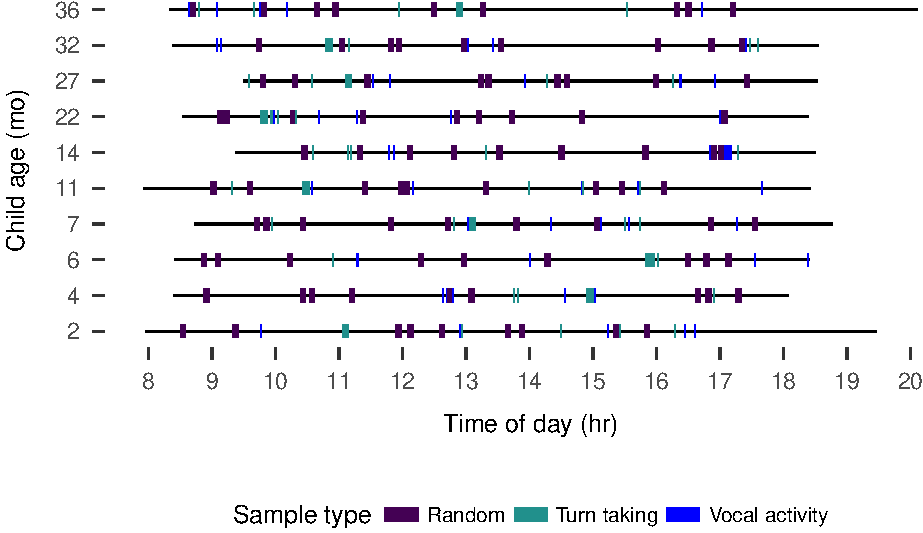
\includegraphics{Tseltal-CLE_files/figure-latex/fig2-1.pdf}
\caption{\label{fig:fig2}By-child estimates of minutes per hour of overheard
speech (left), target-child-directed speech (right). Data are shown for
the random (purple; solid) and turn taking (green; dashed) samples.
Bands on the solid linear trends show 95\% CIs.}
\end{figure}

\subsection{Target-child-directed speech
(TCDS)}\label{target-child-directed-speech-tcds}

The Tseltal children in our study were directly spoken to for an average
of 3.63 minutes per hour in the random sample (median = 4.08; range =
0.83--6.55; \protect\hyperlink{fig2}{Figure 2}). These estimates are
close to those reported for Yucatec Mayan data (Laura A Shneidman \&
Goldin-Meadow, 2012), which are plotted with our data, along with
estimates from a few other populations in
\protect\hyperlink{fig3}{Figure 3} (US/Canada: E. Bergelson et al.,
2018; Tsimane: Scaff, Stieglitz, Casillas, \& Cristia, In preparation;
US urban and Yukatek: Laura A. Shneidman, 2010; Mozambique urban and
rural, and Dutch: Vogt, Mastin, \& Schots, 2015).\footnote{We convert
  the original estimates from Laura A. Shneidman (2010) into min/hr by
  using the median utterance duration in our dataset for all non-target
  child speakers: (1029ms). Note that, though this conversion is far
  from perfect, Yukatek and Tseltal are related languages.}. We modeled
TCDS min/hr in the random clips with a zero-inflated negative binomial
regression, as described above.

\begin{figure}
\centering
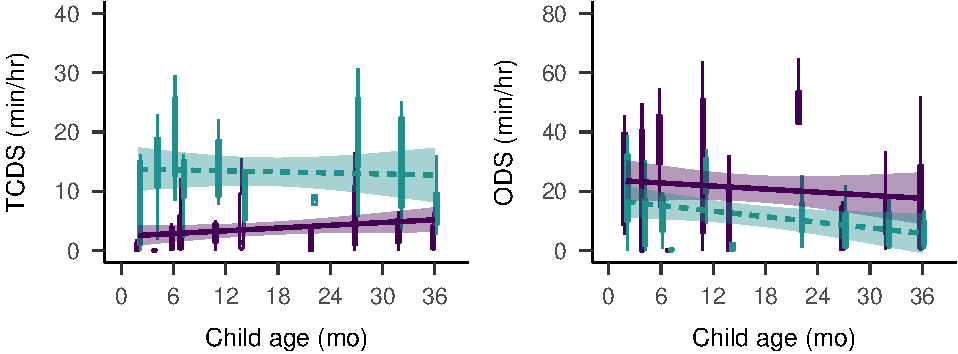
\includegraphics{Tseltal-CLE_files/figure-latex/fig3-1.pdf}
\caption{\label{fig:fig3}TCDS rate reported across different populations,
including both urban (gray) and rural/indigenous (black) samples. Each
point is the average TCDS rate reported for children at the indicated
age, and size indicates number of children sampled (range: 1--26). See
text for references to original studies.}
\end{figure}

The rate of TCDS in the randomly sampled clips was primarily affected by
factors relating to the time of day. The count model showed that,
overall, children were more likely to hear TCDS in the mornings and
evenings than around midday (B = 4.36, SD = 1.93, z = 2.26, p = 0.02).
However, this pattern weakened for older children, some of whom even
heard peak TCDS input around midday, as illustrated in
\protect\hyperlink{fig4}{Figure 4} (B = -5.23, SD = 1.98, z = -2.64, p =
0.01). There were no significant effects of child age, household size,
or number of speakers present, no significant effects in the
zero-inflation model.\footnote{This TCDS zero-inflation did not include
  the number of speakers present or time of day.}

\begin{figure}
\centering
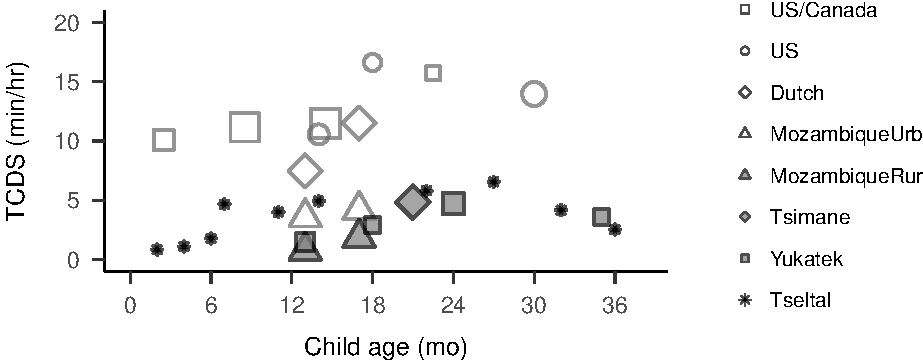
\includegraphics{Tseltal-CLE_files/figure-latex/fig4-1.pdf}
\caption{\label{fig:fig4}TCDS rate heard at different times of day by
children 12 months and younger (left) and 13 months and older (right) in
the randomly selected (purple) and turn-taking (green) clips.}
\end{figure}

In contrast to findings from Laura A Shneidman and Goldin-Meadow (2012)
on Yucatec Mayan, most TCDS in the current data came from adult speakers
(mean = 80.61\%, median = 87.22\%, range = 45.90\%--100), with no
evidence for an increase in proportion TCDS from children with target
child age (correlation between child age and proportion TCDS from
children: Spearman's \emph{rho} = -0.29; \emph{p} = 0.42).

\subsection{Other-directed speech
(ODS)}\label{other-directed-speech-ods}

Children heard an average of 21.05 minutes per hour in the random sample
(median = 17.80; range = 3.57--42.80): that is, 5--6 times as much
speech as was directed to them. We modeled ODS min/hr in the random
clips with a zero-inflated negative binomial regression, as described
above.

The count model of ODS in the randomly selected clips revealed that the
presence of more speakers was strongly associated with more ODS (B =
1.06, SD = 0.09, z = 11.54, p = 0). Additionally, more ODS occurred in
the mornings and evenings (B = 2.72, SD = 1.15, z = 2.37, p = 0.02), and
was also more frequent in large households for older children compared
to younger children (B = 0.33, SD = 0.16, z = 2.01, p = 0.04). There
were no other significant effects on ODS rate, and no significant
effects in the zero-inflation models.\footnote{This ODS count model did
  not include by-child intercepts of time of day and its zero-inflation
  did not include the number of speakers present.}

Other-directed speech may have been so common because there were an
average 3.44 speakers present other than the target child in the
randomly selected clips (median = 3; range = 0--10), and (typically)
more than half of the speakers were adults. However, these estimates are
comparable to North American infants (6--7 months) living in nuclear
family homes (REFS; Elika Bergelson, Amatuni, Dailey, Koorathota, \&
Tor, 2018), so a high incidence of ODS may be common for infants in many
sociocultural contexts.

\begin{figure}
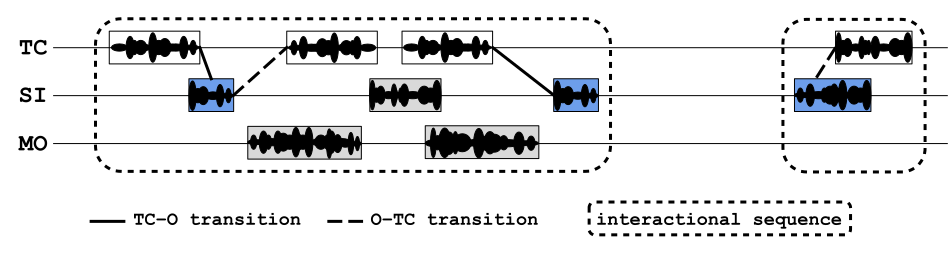
\includegraphics[width=1\linewidth]{Tseltal-CLE_files/TseltalCLE-TurnTimingIllustration} \caption{Illustration of a transcript clip between the target child (TCH), an older sister (SIS), and mother (MOT) in which transitions between the target child and other interlocutors are marked in solid and dashed lines and in which interactional sequences are marked with dotted lines. Light gray boxes indicate TCDS and dark gray boxes indicate ODS.}\label{fig:fig5}
\end{figure}

\subsection{Target-child-to-other turn transitions
(TC--O)}\label{target-child-to-other-turn-transitions-tco}

We detect contingent turn exchanges between the target child and other
speakers based on turn timing \protect\hyperlink{fig5}{Figure 5}. If a
child's vocalization is followed by a target-child-directed utterance
within -1000--2000msec of the end of the child's vocalization (Casillas,
Bobb, \& Clark, 2016; Hilbrink, Gattis, \& Levinson, 2015), it is
counted as a contingent response (i.e., a TC--O transition). We use the
same idea to find other-to-target-child transitions below (i.e., a
target-child-directed utterance followed by a target child vocalization
with the same overlap/gap restrictions). Each target child vocalization
can only have one prompt and one response and each target-child-directed
utterance can maximally count once as a prompt and once as a response
(e.g., in a TC--O--TC sequence, the \enquote{O} is both a response and a
prompt).

Gap and overlap restrictions are based on prior studies of infant and
young children's turn taking (Casillas et al., 2016; Hilbrink et al.,
2015), though the timing margins are increased slightly for the current
dataset because the prior estimates come from relatively short, intense
bouts of interaction in WEIRD parental contexts (see also, e.g., REFS
for studies on contingency with much longer allowed time lapses).

\begin{figure}
\centering
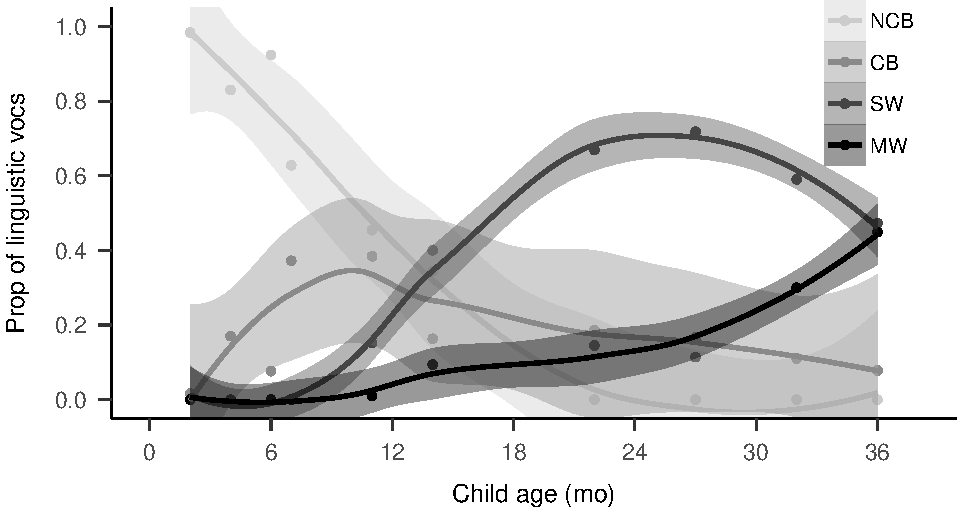
\includegraphics{Tseltal-CLE_files/figure-latex/fig6-1.pdf}
\caption{\label{fig:fig6}By-child estimates of contingent responses per
minute to the target child's vocalizations (left), contingent responses
per minute by the target child to others' target-child-directed speech
(middle), and the average duration of contingent interactional sequences
(right). Each datapoint represents the value for a single clip within
the random (purple; solid) or turn taking (green; dashed) samples. Bands
on the solid linear trends show 95\% CIs.}
\end{figure}

Other speakers responded contingently to the target children's
vocalizations at an average rate of 1.38 transitions per minute (median
= 0.40; range = 0--8.60). We modeled TC--O transtions per minute in the
random clips with a zero-inflated negative binomial regression, as
described above.

The rate at which children hear contingent response from others was
primarily influenced by factors relating to the child's age. Older
children heard more contingent responses then younger children when
there were more speakers present (B = 0.47, SD = 0.22, z = 2.10, p =
0.04). Also, as with the speech quantity measures, younger children
heard more contingent responses in the mornings and evenings while this
effect was less pronounced for older children (B = -6.47, SD = 2.57, z =
-2.52, p = 0.01).There were no other significant effects on TC--O
transition rate, and no significant effects in the zero-inflation model
either.\footnote{This TC--O transition count model did not include
  by-child intercepts of time of day.}

\subsection{Other-to-target-child turn transitions
(O--TC)}\label{other-to-target-child-turn-transitions-otc}

Tseltal children responded contingently to others' target-child
vocalizations at an average rate of 1.17 transitions per minute (median
= 0.20; range = 0--8.80). We modeled O--TC transtions per minute in the
random clips with a zero-inflated negative binomial regression, as
described above.

The rate at which children respond contingently to others (O--TC turn
transitions per minute) was similarly influenced by child age and time
of day: older children were less likely than young children to show peak
response rates in the morning and evening (B = -7.31, SD = 2.62, z =
-2.79, p = 0.01). There were no further significant effects in the count
or zero-inflation models.\footnote{This O--TC transition count model did
  not include by-child intercepts of time of day.}

\subsection{Sequence duration}\label{sequence-duration}

Sequences of interaction include periods of contingent turn taking with
at least one target child vocalization and one target-child-directed
prompt or response from another speaker. We use the same mechanism as
before to detect contingent TC--O and O--TC transitions, but also allow
for speakers to continue with multiple vocalizations in a row (e.g.,
TC--O--O--TC--OTH; \protect\hyperlink{fig5}{Figure 5}. Sequences are
bounded by the earliest and latest vocalization for which there is no
contingent prompt/response, respectively. Each target child vocalization
can only appear in one sequence, and many sequences have more than one
child vocalization. Because sequence durations were not zero-inflated,
we modeled them in the random clips with negative binomial regression.

We detected 311 interactional sequences in the 90 randomly selected
clips, with an average sequence duration of 10.13 seconds (median = 7;
range = 0.56--85.47). The average number of child vocalizations within
these sequences was 3.75 (range = 1--29; median = 3). None of the
predictors significantly impacted sequence duration (all \emph{p}
\textgreater{} 0.09).\footnote{This sequence duration model did not
  include by-child intercepts of time of day.}

\subsection{Peak interaction}\label{peak-interaction}

As expected, the turn-taking clips featured a much higher rate of
contingent turn transitions: the average TC--O transition rate was 7.73
transitions per minute (median = 7.80; range = 0--25) and the average
O--TC rate was 7.56 transitions per minute (median = 6.20; range =
0--26). The interactional sequences were also longer on average: 12.27
seconds (median = 8.10; range = 0.55--61.22).

Crucially, children also heard much more TCDS in the turn-taking
clips---13.28 min/hr (median = 13.65; range = 7.32--20.19)---while also
hearing less ODS---11.93 min/hr (median = 10.18; range = 1.37--24.42).

We modeled each of these five speech environment measures with parallel
models to those used above (with no zero-inflation model for TCDS,
TC--O, and O--TC rates, given the nature of the sample). The impact of
child age, time of day, household size, and number of speakers was
qualitatively similar (basic sample comparisons are visualized in
\protect\hyperlink{fig2}{Figure 2}, \protect\hyperlink{fig3}{Figure 3},
and \protect\hyperlink{fig5}{Figure 5}) between the randomly selected
clips and these peak periods of interaction with the following
exceptions: older children heard significantly less ODS (B = -0.49, SD =
0.19, z = -2.57, p = 0.01), the presence of more speakers significantly
decreased children's response rate to other's vocalizations (B = -0.26,
SD = 0.12, z = -2.19, p = 0.03), and children's interactional sequences
were shorter for older children (B = -0.24, SD = 0.10, z = -2.42, p =
0.02), shorter for children in large households (B = -0.21, SD = 0.10, z
= -2.25, p = 0.02), and longer during peak periods in the mornings and
afternoons (B = 2.77, SD = 1.11, z = 2.50, p = 0.01). Full model outputs
can be compared in the Supplementary Materials.

\subsubsection{Peak minutes in the day}\label{peak-minutes-in-the-day}

\section{Discussion}\label{disc}

\subsection{Future directions}\label{disc-future}

\subsection{Conclusion}\label{disc-conclusion}

\section{Acknowledgements}\label{acknowledgements}

\newpage

\section{References}\label{refs}

\begingroup
\setlength{\parindent}{-0.5in} \setlength{\leftskip}{0.5in}

\hypertarget{refs}{}
\hypertarget{ref-bergelson2018day}{}
Bergelson, E., Amatuni, A., Dailey, S., Koorathota, S., \& Tor, S.
(2018). Day by day, hour by hour: Naturalistic language input to
infants. \emph{Developmental Science}, \emph{XX}, XX--XX.

\hypertarget{ref-bergelsoncasillas2018what}{}
Bergelson, E., Casillas, M., Soderstrom, M., Seidl, A., Warlaumont, A.
S., \& Amatuni, A. (2018). What do north american babies hear? A
large-scale cross-corpus analysis. \emph{Developmental Science},
\emph{XX}, XX--XX.

\hypertarget{ref-R-glmmTMB}{}
Brooks, M. E., Kristensen, K., van Benthem, K. J., Magnusson, A., Berg,
C. W., Nielsen, A., \ldots{} Bolker, B. M. (2017a). glmmTMB balances
speed and flexibility among packages for zero-inflated generalized
linear mixed modeling. \emph{The R Journal}, \emph{9}(2), 378--400.
Retrieved from
\url{https://journal.r-project.org/archive/2017/RJ-2017-066/index.html}

\hypertarget{ref-brooks2017modeling}{}
Brooks, M. E., Kristensen, K., van Benthem, K. J., Magnusson, A., Berg,
C. W., Nielsen, A., \ldots{} Bolker, B. M. (2017b). Modeling
zero-inflated count data with glmmTMB. \emph{bioRxiv}.
doi:\href{https://doi.org/10.1101/132753}{10.1101/132753}

\hypertarget{ref-casillas2016turn}{}
Casillas, M., Bobb, S. C., \& Clark, E. V. (2016). Turn taking, timing,
and planning in early language acquisition. \emph{Journal of Child
Language}, \emph{43}, 1310--1337.

\hypertarget{ref-hilbrink2015early}{}
Hilbrink, E., Gattis, M., \& Levinson, S. C. (2015). Early developmental
changes in the timing of turn-taking: A longitudinal study of
mother--infant interaction. \emph{Frontiers in Psychology},
\emph{6:1492}, 1--12.

\hypertarget{ref-R-base}{}
R Core Team. (2018). \emph{R: A language and environment for statistical
computing}. Vienna, Austria: R Foundation for Statistical Computing.
Retrieved from \url{https://www.R-project.org/}

\hypertarget{ref-scaffIPlanguage}{}
Scaff, C., Stieglitz, J., Casillas, M., \& Cristia, A. (In preparation).
Language input in a hunter-forager population: Estimations from daylong
recordings.

\hypertarget{ref-shneidman2010language}{}
Shneidman, L. A. (2010). \emph{Language input and acquisition in a Mayan
village} (PhD thesis). The University of Chicago.

\hypertarget{ref-shneidman2012language}{}
Shneidman, L. A., \& Goldin-Meadow, S. (2012). Language input and
acquisition in a Mayan village: How important is directed speech?
\emph{Developmental Science}, \emph{15}(5), 659--673.

\hypertarget{ref-smithson2013generalized}{}
Smithson, M., \& Merkle, E. (2013). \emph{Generalized linear models for
categorical and continuous limited dependent variables}. CRC Press: Boca
Raton.

\hypertarget{ref-vogt2015communicative}{}
Vogt, P., Mastin, J. D., \& Schots, D. M. A. (2015). Communicative
intentions of child-directed speech in three different learning
environments: Observations from the netherlands, and rural and urban
mozambique. \emph{First Language}, \emph{35}(4-5), 341--358.

\hypertarget{ref-R-ggplot2}{}
Wickham, H. (2009). \emph{Ggplot2: Elegant graphics for data analysis}.
Springer-Verlag New York. Retrieved from \url{http://ggplot2.org}

\endgroup






\end{document}
